
\subsection*{task 1.1 [10 points] \\[1ex] computing spectral- and singular value decompositions}

In the \texttt{Data} folder for this exercise, you will find the file
\begin{quote}
    \texttt{faceMatrix.npy}
\end{quote}
which contains a data matrix $\mat{X} \in \mathbb{R}^{361 \times 2429}$ whose columns $\vec{x}_i$ represent tiny face images of size $19 \times 19$ pixels. To read this matrix into memory and check its size, you may use
\begin{python}
matX = np.load('faceMatrix.npy').astype('float')
m, n = matX.shape
print (m, n)
\end{python}
To have a look at one of the images it contains, say $\vec{x}_{15}$, you may use this
\begin{python}
vecX = matX[:,14].reshape(19,19)
plt.imshow(vecX, cmap='gray')
plt.xticks([])
plt.yticks([])
plt.show()
\end{python}
\vspace{2cm}





Having read matrix $\mat{X}$ into memory, here is what you are supposed to do
\begin{enumerate}
\item normalize $\mat{X}$ such that its column mean is $\vec{0}$
%%%%%
%%%%%
%%%%% enter your code into the following environment
%%%%%
%%%%%
\begin{python}
# normalize the data matrix such that the column mean is zero
# by simply subtracting the mean of each column
X -= X.mean(axis=0, keepdims=True)
\end{python}
%%%%%
%%%%%
%%%%%
%%%%%
%%%%%
\item compute $\mat{C} = \mat{X} \trn{\mat{X}}$ \\ \textbf{NOTE:} we deliberately omit the scaling factor of $\frac{1}{n}$
\item compute the spectral decomposition $\mat{C} = \mat{U} \mat{\Lambda} \,\trn{\mat{U}}$ using \keyword{la.eig}
\item compute the spectral decomposition $\mat{C} = \mat{U} \mat{\Lambda} \,\trn{\mat{U}}$ using \keyword{la.eigh}
\item compare the eigenvalues you obtain from these two approaches; what do you observe ?
\color{blue} \\[1ex]
%%%%%
%%%%%
%%%%% enter your discussion here
%%%%%
%%%%%
Up to permutation the two spectra are exaclty the same (see figure \ref{fig:eig_vs_eigh}). The reason for the different permutations is simply that \keyword{la.eigh} guarantees that the eigenvalues are sorted whereas \keyword{la.eig} doesn't. Also it might happen that some of the elements have flipped signs but we didn't observe this here.

\begin{figure}
    \centering
    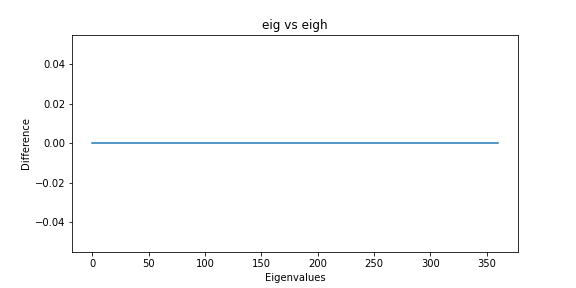
\includegraphics[width=\textwidth]{Ex_01/Figures/eig-vs-eigh.png}
    \caption{Difference of the sorted eigenvalues computed by the two methods. The x-axis lists all the eigenvalues of the matrix $C$ and the y-axis shows the difference of the corresponding values. Really not much to see here.}
    \label{fig:eig_vs_eigh}
\end{figure}
%%%%%
%%%%%
%%%%%
%%%%%
%%%%%
\color{black}
\item compute the singular value decomposition $\mat{X} = \mat{U} \mat{\Sigma} \trn{\mat{V}}$ using \keyword{la.svd}
\item square the resulting singular values and compare them to the eigenvalues you found above; what do you observe ?
\color{blue} \\[1ex]
%%%%%
%%%%%
%%%%% enter your discussion here
%%%%%
%%%%%
As the theory suggests we observe that the squared singular values equal the eigenvalues of the matrix $C$ (again up to permutation). Nevertheless we see distortions between the two sets (see figure \ref{fig:eigh_vs_svd}). This is probably due to numerical error, since \keyword{la.svd} doesn't directly compute the eigenvalues but their square root. The magnitude of the eigenvalues that show differences also support our hypothesis. Still the differences are negligible.

\begin{figure}
    \centering
    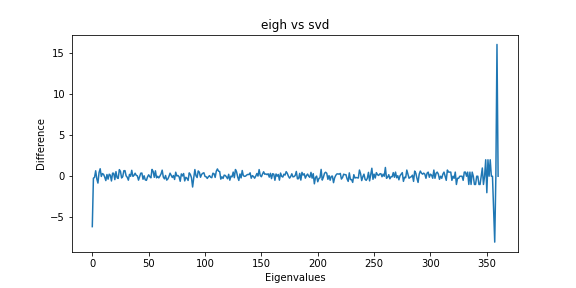
\includegraphics[width=\textwidth]{Ex_01/Figures/eigh-vs-svd.png}
    \caption{Difference between the eigenvalues computed by \keyword{la.eigh} and \keyword{la.svd}. Other than before there actually are differences between the two spectra. But w.r.t to the magnitude of the values, the error is negligible. Note that the eigenvalues are sorted in ascending order.}
    \label{fig:eigh-vs-svd}
\end{figure}
%%%%%
%%%%%
%%%%%
%%%%%
%%%%%
\color{black}
\item create a plot of the three spectra you just computed; do you get any warnings or error messages ?
%%%%%
%%%%%
%%%%% enter plot here, i.e. replace "placeholder.pdf" by the name of the graphics file you created
%%%%%
%%%%%
\begin{center}
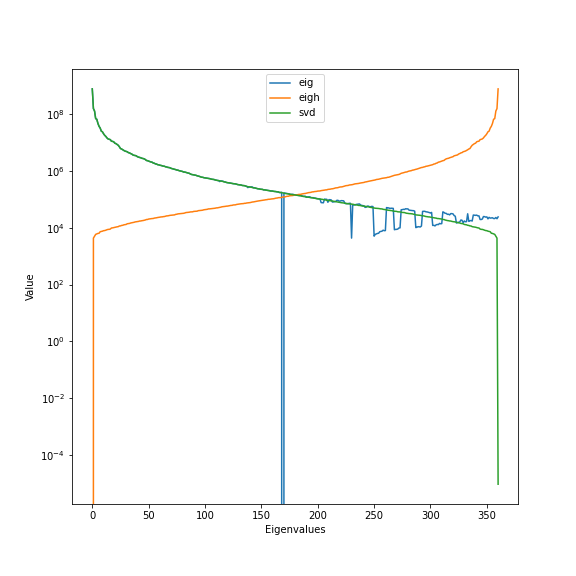
\includegraphics[width=0.75\textwidth]{Ex_01/Figures/eig.png}
\end{center}
%%%%%
%%%%%
%%%%%
%%%%%
%%%%%
\end{enumerate}

